% =============================================================================
%  avance_socioformador.tex - presentacion breve de avance (issue #64)
%  VERSION SIMPLE: lenguaje llano, sin jerga estadistica. Ver tambien
%  avance_socioformador_tecnico.tex (misma estructura, cifras identicas,
%  redaccion tecnica) para comparar las dos opciones.
%
%  NO es la presentacion final de entrega: es un medio para mostrarle al
%  socioformador el avance tras el cambio de objetivo y recibir
%  retroalimentacion. Compila independiente de reports/ (misma carpeta de
%  figuras, via \graphicspath, para no duplicar archivos).
%
%  Estructura (3 diapositivas de contenido):
%    1. Objetivo y tratamiento de los datos (los componentes se resumen)
%    2. Los dos modelos, juntos
%    3. Conclusiones
%
%  Cifras tomadas de reports/secciones/objetivo_tecnicas.tex,
%  reports/secciones/pca.tex, reports/secciones/regresion_logistica.tex
%  (incluida su subseccion "Conclusiones") y docs/log_limpieza.md.
%
%  Compilar desde esta carpeta:   latexmk avance_socioformador.tex
% =============================================================================

\documentclass{beamer}

\usetheme{Madrid}
\usecolortheme{default}

\usepackage[T1]{fontenc}
\usepackage[utf8]{inputenc}
% Igual que reports/main.tex: es-nodecimaldot evita que babel convierta
% los puntos decimales en comas dentro de modo matematico.
\def\spanishoptions{es-tabla,es-nodecimaldot,es-noquoting}
\usepackage[spanish]{babel}
\usepackage{enumitem}

% Reutiliza las figuras ya generadas para el reporte; no se duplican aqui.
\graphicspath{{../reports/figuras/}}

\setbeamertemplate{navigation symbols}{}
\setbeamertemplate{caption}[numbered]

% El titulo coincide con el de reports/main.tex; el subtitulo es la segunda
% linea (\large) de ese mismo titulo. La distincion entre esta version y la
% otra NO va en la portada: vive en el nombre del archivo y en el README.
\title[Excedencias de ozono en el AMM]{Discriminación de excedencias de ozono
día-estación bajo el umbral de 51 ppb de la NOM-020-SSA1-2021}
\subtitle{Comparación de análisis discriminante lineal y regresión logística en
15 estaciones del SIMA, Área Metropolitana de Monterrey}
\author[Equipo 102.07]{Angel Luna \and Jenaro Alcaraz \and Emilia Rico \and
Mar Fernández \and Sofía Fernández}
\institute[MA2003B --- 102.07]{Instituto Tecnológico y de Estudios Superiores
de Monterrey \\ MA2003B --- Grupo 102.07}
\date{\today}

\begin{document}

\begin{frame}
  \titlepage
\end{frame}

% -----------------------------------------------------------------------
% Diapositiva 1: objetivo y tratamiento de los datos.
% Fuente: reports/secciones/objetivo_tecnicas.tex, reports/secciones/pca.tex
% y docs/log_limpieza.md (secciones 3 y 5).
% -----------------------------------------------------------------------
\begin{frame}{Qué buscamos y cómo tratamos los datos}
  \scriptsize

  \textbf{El objetivo.} Identificar, día por día y por estación, cuándo el aire del Área Metropolitana de Monterrey superó el límite de ozono de la norma oficial (\textbf{51 ppb}, meta a cinco años de la NOM-020-SSA1-2021), a partir de los contaminantes y el clima de ese mismo día. El modelo \textbf{explica} qué acompaña esos episodios; no \textbf{predice} los siguientes.
  \vspace{2pt}

  \begin{columns}[T]
    \begin{column}{0.62\textwidth}
      \textbf{Qué hicimos con los datos}
      \begin{itemize}[itemsep=1pt,topsep=1pt,parsep=0pt,leftmargin=*]
        \item \textbf{Huecos}: rellenamos el \textbf{1.67\,\%} de los datos
          faltantes uniendo la medición anterior con la siguiente, solo cuando
          el hueco dura 3 horas o menos. Los paros largos se dejan vacíos.
        \item \textbf{Valores extremos: se detectan, pero se conservan.}
          Queremos justamente clasificar los días de excedencia; quitar los
          valores altos nos quitaría la información más relevante.
        \item \textbf{Lo que sí se elimina son errores del equipo}: el código
          de dato ausente del registrador ($-9999$), los topes de saturación
          del sensor (999, 1000, 1001) y las lecturas fuera del rango físico
          que el aparato puede medir. Menos del 0.02\,\% de los datos.
      \end{itemize}
      \vspace{1pt}
      \textbf{Los tres ejes.} Muchas de las 15 variables se mueven juntas
      (\texttt{NO} y \texttt{NOX} casi como una sola), así que las resumimos en
      tres ejes ---quema de combustibles, qué tan soleado y seco está el día, y
      qué tanto se estanca el aire--- que conservan el \textbf{55.9\,\%} de esa
      información y alimentan los modelos.
    \end{column}
    \begin{column}{0.38\textwidth}
      \centering
      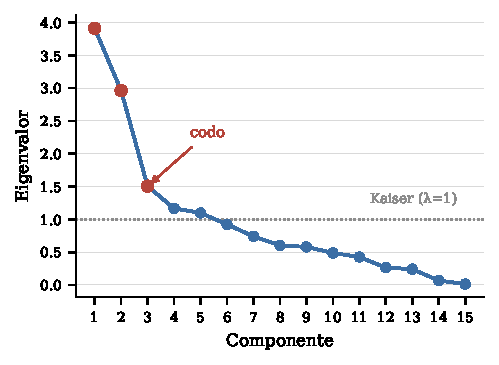
\includegraphics[width=\linewidth]{pca_scree.pdf}

      \scriptsize Información que aporta cada eje.
    \end{column}
  \end{columns}
\end{frame}

% -----------------------------------------------------------------------
% Diapositiva 2: los dos modelos en una sola diapositiva.
% Fuente: reports/secciones/regresion_logistica.tex.
% -----------------------------------------------------------------------
\begin{frame}{Los dos modelos que probamos}
  \scriptsize

  \textbf{Cómo los evaluamos.} Ambos aprenden con los años 2021--2024 y se
  califican con 2025, fechas que no vieron durante el ajuste.
  \vspace{3pt}

  \begin{columns}[T]
    \begin{column}{0.58\textwidth}
      \textbf{Regresión logística.} Estima la probabilidad de que un día
      exceda el límite y dice cuánto pesa cada condición.
      \begin{itemize}[itemsep=1pt,topsep=2pt,parsep=0pt,leftmargin=*]
        \item Distingue los días con y sin excedencia con una calificación
          de \textbf{0.893} sobre 1, muy por encima de la meta de 0.75.
        \item Detecta el \textbf{83.1\,\%} de las excedencias reales y
          descarta bien el \textbf{82.4\,\%} de los días limpios.
        \item Lo que más empuja hacia la excedencia es la
          \textbf{primavera}, seguida del otoño y de las zonas Noroeste y
          Suroeste.
      \end{itemize}
      \vspace{2pt}
      \textbf{Discriminante lineal.} La otra técnica; parte de supuestos
      más fuertes sobre la forma de los datos.
      \begin{itemize}[itemsep=1pt,topsep=2pt,parsep=0pt,leftmargin=*]
        \item Uno de esos supuestos no se cumple: los días de excedencia
          varían menos que los demás.
        \item Aun así llega a la misma calificación de \textbf{0.893},
          detectando el \textbf{84.5\,\%} de las excedencias y acertando en
          el \textbf{81.1\,\%} de los días limpios.
      \end{itemize}
      \vspace{2pt}
      \textbf{Comparación.} Los dos coinciden en el \textbf{98.1\,\%} de
      sus decisiones y una prueba estadística no encuentra diferencia real
      entre ellos.
    \end{column}
    \begin{column}{0.42\textwidth}
      \centering
      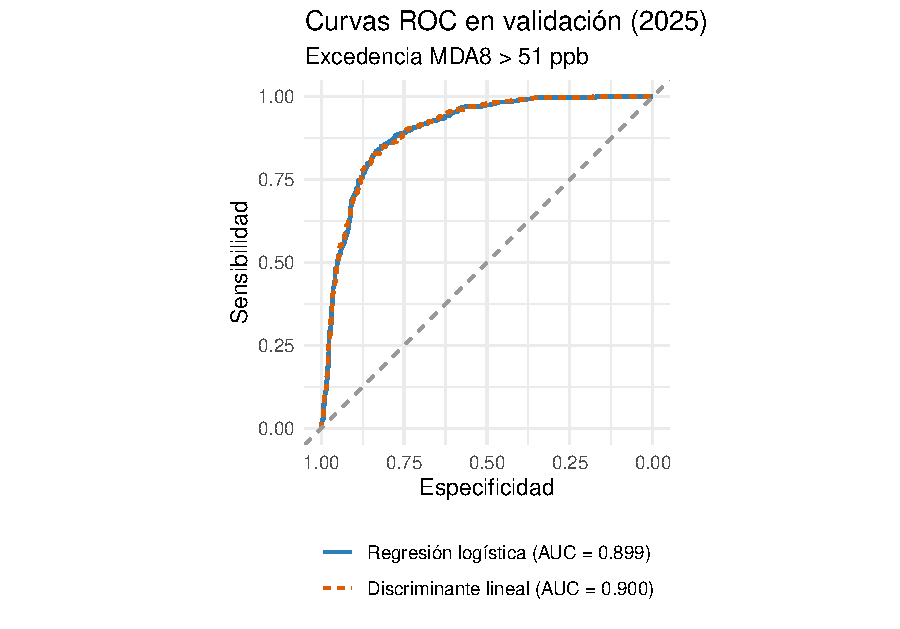
\includegraphics[width=\linewidth]{roc_modelos.pdf}

      \scriptsize Las dos curvas se superponen casi por completo.
    \end{column}
  \end{columns}
\end{frame}

% -----------------------------------------------------------------------
% Diapositiva 3: conclusiones.
% Son las mismas cuatro de reports/secciones/regresion_logistica.tex,
% subseccion "Conclusiones", en lenguaje llano.
% -----------------------------------------------------------------------
\begin{frame}{Lo que concluimos hasta ahora}
  \footnotesize

  \begin{enumerate}[label=\textbf{\roman*.},itemsep=6pt,topsep=2pt,parsep=0pt,leftmargin=*]
    \item \textbf{Los dos modelos llegan a lo mismo.} Aciertan casi igual,
      lo que indica que la frontera entre días de excedencia y días limpios
      la marcan los datos y no el método elegido.

    \item \textbf{La temporada del año manda sobre todo lo demás.} Un día
      de primavera tiene cinco veces más posibilidades de excedencia que
      uno de invierno en igualdad de condiciones. La excedencia de ozono es,
      ante todo, un fenómeno estacional.

    \item \textbf{Hay algo del territorio que no estamos midiendo.} El
      Noroeste y el Suroeste tienen alrededor de \textbf{tres veces} las
      posibilidades del Noreste aun con el mismo clima: algo propio de esas
      zonas, que las variables disponibles no capturan, las vuelve zonas de
      riesgo.

    \item \textbf{El calendario laboral casi no influye.} Solo el domingo
      muestra un efecto, y modesto; sábados y días festivos no se
      distinguen de un día laborable. Montar un estudio sobre el ``efecto
      fin de semana'' con estos datos daría un resultado débil.
  \end{enumerate}
\end{frame}

\end{document}
